\documentclass{article}

\usepackage[margin=1in]{geometry}
\usepackage{amsmath,amsthm,amssymb}
\usepackage{bbm,enumerate,mathtools,multicol}
\usepackage[hidelinks]{hyperref}
\usepackage{tikz}
\usetikzlibrary{matrix, arrows}

\newenvironment{problem}[2][Problem]{\begin{trivlist}
\item[\hskip \labelsep {\bfseries #1}\hskip \labelsep {\bfseries #2.}]}{\end{trivlist}}
\newenvironment{solution}[1][Solution.]{\begin{trivlist}
\item[\hskip \labelsep {\bfseries #1}]}{\end{trivlist}}
\newenvironment{problempart}[1]{\begin{trivlist}\item[\textbf{Part #1.}]}{\end{trivlist}}

\begin{document}

\title{Combinatorics: Homework 1}
\author{Peter Kagey}

\maketitle

% -----------------------------------------------------
% First problem
% -----------------------------------------------------
\begin{problem}{5} \text{} \\
  Let the maps $f_0, f_1\colon X \rightarrow Y$ be homotopic by a homotopy
  $H\colon X \times [0,1] \rightarrow Y$, and let $\gamma$ be the path from
  $y_0 = f_0(x_0)$ to $z_0 = f_1(x_0)$ defined by $\gamma(t) = H(x_0, t)$.
  \begin{enumerate}[(a)]
    \item Let $\alpha\colon[0,1]\rightarrow X$ be a loop in $X$ based at $x_0$.
    What is the path homotopy between the paths $f_0 \circ \alpha$ and
    $\gamma * ((f_1 \circ \alpha) * \bar\gamma)$?
    \item Show that the homomorphisms
    $f_{0*}\colon \pi_1(X; x_0) \rightarrow \pi_1(Y; y_0)$ and
    $f_{1*}\colon \pi_1(X; x_0) \rightarrow \pi_1(Y; z_0)$ (induced by $f_0$ and
    $f_1$ respectively) are related by the property that
    $f_{0*} = T_\gamma \circ f_{1*}$, where $T_\gamma$ is the usual change of
    basepoint isomorphism.
  \end{enumerate}
\end{problem}

\begin{proof} \text{} \\
  \begin{enumerate}[(a)]
    \item
    \begin{multicols}{2}
      Here's the idea in a picture:\\
      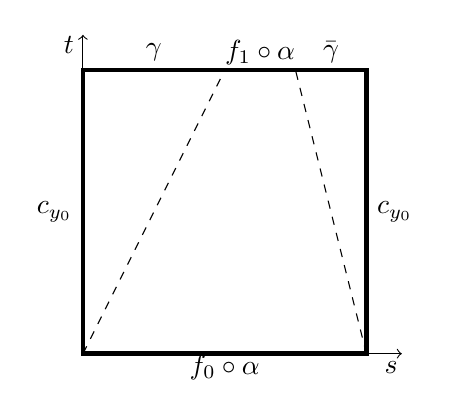
\begin{tikzpicture}[scale = 0.9]
        \draw[ultra thick] (0,0) rectangle (4,4);
        \draw[->] (0,0)--(0,4.5);
        \draw[->] (0,0)--(4.5,0);
        \draw[dashed] (0,0)--(2,4);
        \draw[dashed] (4,0)--(3,4);
        \node at (-0.2,4.35) {$t$};
        \node at (4.35,-0.2) {$s$};
        \node at (1,4.25) {$\gamma$};
        \node at (2.5,4.25) {$f_1\circ\alpha$};
        \node at (3.5,4.25) {$\bar\gamma$};
        \node at (2, -0.2) {$f_0\circ\alpha$};
        \node at (-0.4, 2) {$c_{y_0}$};
        \node at (4.4, 2) {$c_{y_0}$};
      \end{tikzpicture}\\
      Here's the idea as a formula:
      \\\vspace{0.7cm}\\
      \[
        H(s, t) = \begin{cases}
          \gamma(2s) & 0 \leq s \leq \frac{1}{2}t \\
          \displaystyle H\left(\alpha\left(\frac{s - t/2}{1 - 3t/4}\right), t\right) & \frac{1}{2}t \leq s \leq 1 - \frac{1}{4}t \\
          \gamma(4-4s) & 1 - \frac{1}{4}t \leq s \leq 1 \\
        \end{cases}
      \]
    \end{multicols}
  Here's an explanation of why the formula is continuous: the three piecewise
  defined parts are compositions of continuous functions and so are continuous.
  So by the pasting lemma, it is enough to check that \begin{enumerate}[(i)]
    \item when $s=0$, $H(0, t) = \gamma(0) = y_0$;
    \item when $s = \frac{1}{2}t$, the first function evaluates to $\gamma(t)$ and the second to $H(\alpha(0),t) = H(x_0,t)$;
    \item when $s = 1 - \frac{1}{4}t$, the second function evalues to $H(\alpha(1),t) = H(x_0,t)$ and the third to $\gamma(t)$; and
    \item when $s=1$, $H(1, t) = \gamma(0) = y_0$.
  \end{enumerate}
  \item To check the property that $f_{0*} = T_\gamma \circ f_{1*}$, it is
  enough to show that the image of $[\alpha] \in \pi_1(X, x_0)$ under both
  functions are equal. The maps are, respectively, \[
    [\alpha] \xmapsto{f_{0*}} [f_0 \circ \alpha]
    \hspace{1.2cm}\text{and}\hspace{1.2cm}
    [\alpha] \xmapsto{T_\gamma \circ f_{1*}} [\gamma * (f_1 \circ \alpha) * \bar\gamma].
  \]
  But the paths $f_0 \circ \alpha$ and $\gamma * (f_1 \circ \alpha) * \bar\gamma$
  have already been shown to be homotopic by the homotopy $G$ described in part
  (a). Thus $[f_0 \circ \alpha] = [\gamma * (f_1 \circ \alpha) * \bar\gamma]$
  and $f_{0*} = T_\gamma \circ f_{1*}$.
\end{enumerate}
\end{proof}
\pagebreak
% -----------------------------------------------------
% Second problem
% -----------------------------------------------------
\begin{problem}{2} \text{} \\
  Let $X$ be a metric space with metric $d_0$, and pick two points
  $x_0, y_0 \in X$. Let $\Omega_{x_0y_0}X$ denote the space of paths
  $\alpha\colon[0,1]\rightarrow X$ going from $x_0$ to $y_0$. Endow
  $\Omega_{x_0y_0}X$ with the distance \[
    d_1(\alpha, \beta) = \sup_{t\in[0,1]} d_0(\alpha(t), \beta(t))
  \]
  \begin{enumerate}[a.]
    \item Let $H\colon[0,1]\times[0,1]\rightarrow X$ be a path homotopy from
    $\alpha \in \Omega_{x_0y_0}X$ to $\beta \in \Omega_{x_0y_0}X$. For every
    $t \in [0,1]$, let $h_t \in \Omega_{x_0y_0}X$ be the path defined by
    $h_t(s) \coloneqq H(t, s)$.
    \\
    Show that the map $h\colon[0,1]\rightarrow\Omega_{x_0y_0}X$ defined by
    $h(t) = h_t$ is a path in  $\Omega_{x_0y_0}X$ going from $h(0) = \alpha$ to
    $ h(1) = \beta$.
    \item Conversely, let $h\colon[0,1]\rightarrow\Omega_{x_0y_0}$ be a path going
    from $h(0)=\alpha$ to $h(1)=\beta$ in $\Omega_{x_0y_0}$. Define
    $H\colon[0,1]\times[0,1]\rightarrow X$ by the property that $H(s,t)=h_t(s)$
    where $h_t = h(t)$.
    \\
    Show that $H$ is a path homotopy from $\alpha$ to $\beta$.
  \end{enumerate}
\end{problem}

\begin{solution} \text{} \\
\end{solution}
\pagebreak
% -----------------------------------------------------
% Third problem
% -----------------------------------------------------
\begin{problem}{3} \text{} \\
  Let $f\colon X\rightarrow Y$ be a map such that there exists maps
  $h,k\colon Y \rightarrow X$ such that $h\circ f \simeq \operatorname{Id}_X$,
  and $f \circ k \simeq \operatorname{Id}_Y$. Show that $f$ is a homotopy
  equivalence, in the sense that there exists a single map
  $g\colon Y \rightarrow X$ such that
  $g \circ f \simeq \operatorname{Id}_X$ and
  $f \circ g \simeq \operatorname{Id}_Y$.
\end{problem}

\begin{solution} \text{} \\
\end{solution}
\end{document}
